\chapter{急性肝衰竭}

\section{前沿学术综述}

急性肝衰竭(acute liver
failure,ALF)是由于药物、感染、中毒等各种因素导致的急性肝细胞坏死或肝细胞器功能严重障碍导致的临床综合征。常发生于正常个体,表现为肝功能的迅速恶化,并导致精神异常及凝血障碍。在我国,约90%的患者是由于急性重型肝炎所致,在欧美国家,多数因药物中毒所致,仍有部分病例原因尚不清楚
\protect\hyperlink{text00019.htmlux5cux23ch1-18}{\textsuperscript{{[}1{]}}}
\textsuperscript{,}
\protect\hyperlink{text00019.htmlux5cux23ch2-18}{\textsuperscript{{[}2{]}}}
。ALF的自然急性肝衰竭多数发生于年轻人,具有较高发病率和病死率,如果不接受肝移植,其生存率不超过15%。

尽管不同原因导致的急性肝衰竭具有一定异质性,但由于肝细胞急性坏死引起的疾病过程具有共同的临床表现。经过几十年的研究,目前仍无对所有急性肝衰竭患者确实有效的药物或治疗方法,多数急性肝衰竭患者均伴有不同程度循环系统紊乱,因此可能影响全身或局部血液动力学的药物引起众多学者的兴趣,其中前列腺素在一些研究中显示出良好前景,但也有研究认为临床价值不大。N---乙酰---半胱氨酸对脓毒性休克患者具有改善肝脏血流和功能的作用,但是当前的证据也不支持对所有急性肝衰竭患者治疗有效,仍需进一步研究
\protect\hyperlink{text00019.htmlux5cux23ch3-18}{\textsuperscript{{[}3{]}}}
\textsuperscript{~}
\protect\hyperlink{text00019.htmlux5cux23ch5-18}{\textsuperscript{{[}5{]}}}
。

目前对于急性肝衰竭的治疗仍是在针对病因治疗的同时加强监测和支持,但目前尚无大规模随机对照临床研究结果,仍然缺乏标准化重症监测及治疗方案。一般认为对于肝损伤尚无凝血功能明显异常和脑病的患者可收住内科病区,出现意识状态改变时需立即转入重症医学科,保持患者出入量平衡、有效控制颅内压、纠正凝血紊乱、维持血液动力学稳定和代谢参数正常;监测及防治感染、消化道出血;保证各种营养合理供给。动态监测凝血指标、血常规、生化指标(包括血糖、转氨酶和胆红素等)、动脉血气分析等。严密的器官监测及支持对改善急性肝衰竭患者预后十分重要。

肝脏支持系统的应用对维持患者生命,帮助其渡过难关,以争取时间寻找供肝进行肝移植,或是创造条件使肝脏功能得以自身恢复,起到十分重要的桥梁作用
\protect\hyperlink{text00019.htmlux5cux23ch6-18}{\textsuperscript{{[}6{]}}}
\textsuperscript{,}
\protect\hyperlink{text00019.htmlux5cux23ch7-18}{\textsuperscript{{[}7{]}}}
。早期肝脏支持系统主要以解毒功能为主,如血液灌流、血液透析/滤过等。用树脂、活性炭等材料进行血液灌流,可有效吸附肝衰竭患者血液中的毒性物质,是早期人工肝支持的常用方法。但由于这些吸附材料与血液生物相容性较差,临床应用副反应大。最近采用活性炭微囊化技术、改良血浆灌流等,避免了活性炭与血细胞直接接触,从而减少了不良反应。但由于吸附材料本身选择性较差,在去除患者体内毒性物质的同时,也吸附了一些机体有用的物质,故虽可显著改善重型肝炎等肝衰竭患者的肝性脑病症状,但病死率并未明显下降。目前主要利用其解毒尤其是吸附胆红素的作用与其他人工肝联合使用或用于治疗重型肝炎。国外最近推出一种新型吸附剂型血液治疗系统(Biologic-DT),采用精制粉末炭、阳离子交换剂、大分子溶剂等组成混合悬液状吸附剂,具有较强的毒物吸附作用,能有效地治疗药物中毒引起的肝衰竭。应用目前通用的聚丙烯腈膜进行血液透析,能有效地去除尿素、肌酐及无机磷酸盐等小分子物质,但对中、大分子物质清除率较低,故仅用于急性肝衰竭同时伴肾衰竭的治疗。新近采用新型膜材料三醋酸纤维膜及聚甲基丙烯酸甲醋膜制成空心纤维血液透析滤过器,其效率为聚丙烯腈膜的3倍,有研究发现能使爆发性肝炎患者意识恢复率达到90%,并改善存活率
\protect\hyperlink{text00019.htmlux5cux23ch8-18}{\textsuperscript{{[}8{]}}}
\textsuperscript{,}
\protect\hyperlink{text00019.htmlux5cux23ch9-18}{\textsuperscript{{[}9{]}}}
。

近年来,生物型人工肝技术取得了长足的进步,与机械性人工肝单纯清除体内毒素不同,生物人工肝不仅能通过对毒素的代谢转化清除毒素,而且能合成生物活性物质如凝血因子等参与机体功能活动,并调节体内血糖等代谢活动。由于目前生物人工肝技术尚不成熟,故一般与机械性人工肝联合使用,以达到更全面的肝脏功能的支持作用
\protect\hyperlink{text00019.htmlux5cux23ch10-18}{\textsuperscript{{[}10{]}}}
\textsuperscript{,}
\protect\hyperlink{text00019.htmlux5cux23ch11-18}{\textsuperscript{{[}11{]}}}
。生物人工肝技术的心脏部位是生物反应器,它由许多条中空纤维毛细管构成,患者的血浆经此流过被保温、氧合和分离,在毛细管外有许多肝细胞,或是单独存在或是与胶原的微载体小粒结合在一起。肝细胞来源最好是用人的肝细胞,但人肝细胞难培养,其表型常不稳定,很快失去肝特征性基因表达。因此目前的技术主要使用其他种系的肝细胞,比如猪肝细胞,其优点是易于低温保存,避免因长时间细胞培养带来的昂贵成本和受污染的风险。最早应用猪肝细胞依赖的生物人工肝技术是1996年由Demetrious及其同事们一起研制成功的,并将此技术用于12例急性肝衰竭患者,持续治疗21~96小时,其中11例患者Ⅳ级肝性脑病有好转,颅内压及大脑灌注压明显改善,血氨、胆红素下降,成功过渡至接受肝移植,但其凝血酶原时间未有改善。

欧美的一些研究机构也进行了一系列多中心随机对照试验
\protect\hyperlink{text00019.htmlux5cux23ch11-18}{\textsuperscript{{[}11{]}}}
\textsuperscript{~}
\protect\hyperlink{text00019.htmlux5cux23ch13-18}{\textsuperscript{{[}13{]}}}
,其中用生物人工肝治疗10例急性肝衰竭,患者经过治疗后血清胆红素水平下降,血氨改变不明显,颅内压及意识水平有明显改善,尤其在因扑热息痛所致肝损伤的患者中更为明显,但蛋白质合成功能无改善,5例患者血小板、纤维蛋白原减少,产生出血的并发症,个别患者发生短暂的血液动力学不稳定。尽管如此,最后所有患者都过渡到肝移植,有8例肝移植患者存活达18个月,生物人工肝组存活>30天者为71%,对照组为62%。去除肝移植接受时间等影响因素,显示了用生物人工肝治疗后病死率降低47%(\emph{P}
=0.03)。另一个依赖肝胚胎细胞的体外肝支持系统是由Sussman及其同事研制的,共治疗24例急性肝衰竭患者,没有引起凝血异常或血流动力学不稳定。体外肝支持系统组经6小时治疗后血氨、血清胆红素水平下降,半乳糖清除率改善,生长激素水平升高,但存活率未有改善。

迄今为止,国际上已有多种不同的肝脏支持系统处于实验及临床研究阶段,尚未得到肯定的临床疗效证据。不过,研究发现,当进行异位或部分肝移植手术时,原来部分肝细胞可以恢复功能,但是恢复过程需要数周或数月的时间,在这段时间需要肝脏替代装置来维持功能,也就是说从长远来看,肝脏支持系统是需要的,它提供了一种肝脏功能替代的有效方法,在一定程度上纠正代谢紊乱、毒素堆积进一步损伤肝细胞的恶性循环,保护了濒临死亡的肝细胞,促进剩余肝脏细胞的再生,并降低体内内毒素及炎性因子水平,改善器官功能,提高急性肝衰竭患者的存活率,并为肝脏移植提供时机,成为治疗急性肝脏功能衰竭的最有效的手段。

对于肝细胞无法大量再生的患者,肝移植是目前唯一有效的治疗措施。重视查找和处理急性肝衰竭的病因对提高存活率也很有帮助。据报道,急性肝衰竭患者移植后的短期存活率高达80%~90%,不过只有29%的急性肝衰竭患者进行了移植手术,列入等待肝移植名单的患者中有10%~40%在等待肝源期间死亡。活体肝移植可以一定程度缓解肝源不足,但其开展也受到各个方面的限制。尽管肝脏移植已经取得了显著的临床疗效,但该领域仍有许多问题有待解决,目前研究的主要方向在于理想、充足供体的供应、保存方法的改进、异种器官移植的可行性、免疫抑制技术的改进等,深入探讨有效肝脏支持或其他顺利过渡到肝移植的方法以及对于急性肝衰竭准确预后评分系统,仍是未来研究的主要方向。

\section{临床问题}

\subsection{急性肝衰竭的病因与临床特征}

\subsubsection{急性肝衰竭的病因有哪些?}

引起急性肝衰竭的病因复杂。不同地区病因不尽相同,明确病因有助于诊断和判断预后,不同病因所致肝衰竭在表现、预后、疗效等方面不尽一致,欧美国家以药物(如乙酰氨基酚)损伤为主;我国则以病毒(主要是乙型肝炎病毒)感染引起的急性肝衰竭较为多见。

(1)嗜肝病毒感染 在我国,急性肝衰竭85%~95%为病毒感染所致,所有嗜肝病毒都能引起急性肝衰竭。常见的肝炎病毒如乙型肝炎病毒、丙型肝炎病毒及丁型肝炎病毒引起的急性肝衰竭相对较多,甲型肝炎病毒、戊型肝炎病毒引起者相对较少,非肝炎病毒以巨细胞病毒、EB病毒及单纯疱疹病毒引起的肝炎较常见
\protect\hyperlink{text00019.htmlux5cux23ch14-18}{\textsuperscript{{[}14{]}}}
\textsuperscript{,}
\protect\hyperlink{text00019.htmlux5cux23ch15-18}{\textsuperscript{{[}15{]}}}
。急性病毒性肝炎发生急性肝衰竭者少于1%。

(2)损肝药物 损肝药物种类繁多,药源性急性肝衰竭的发生率有增高趋势,占急性肝衰竭的2.9%
\protect\hyperlink{text00019.htmlux5cux23ch16-18}{\textsuperscript{{[}16{]}}}
\textsuperscript{,}
\protect\hyperlink{text00019.htmlux5cux23ch17-18}{\textsuperscript{{[}17{]}}}
。引起急性肝衰竭的药物主要包括抗结核药(对氨基水杨酸、异烟肼、利福平、吡嗪酰胺)、大剂量四环素、对乙酰氨基酚、非甾体类抗炎药等。据报道,对乙酰氨基酚过量是英国急性肝衰竭的主要病因;印度4.5%的急性肝衰竭由抗结核药引起;日本25%的特发性急性肝衰竭系服用乙肼苯哒嗪(Ecarazine)所致。对乙酰氨基酚中毒患者中有69%符合诊断标准(每天对乙酰氨基酚用量>4g),83%的患者符合血清对乙酰氨基酚水平诊断标准,92%的患者转氨酶水平≥3500IU/L,41%的患者有自杀倾向,55%的患者为无意服药过量(多次服药、有疼痛症状而没有自杀倾向),与麻醉镇痛药联用导致急性肝衰竭的患者占38%。应注意虽然患者按处方服药仍有可能中毒。

(3)毒物中毒 种类也很多,如毒蕈、四氯化碳、磷等。美国和法国报道,每年都有业余蘑菇采集者因毒蕈中毒引起急性肝衰竭而死亡
\protect\hyperlink{text00019.htmlux5cux23ch18-18}{\textsuperscript{{[}18{]}}}
\textsuperscript{~}
\protect\hyperlink{text00019.htmlux5cux23ch20-18}{\textsuperscript{{[}20{]}}}
,这类毒素最常见的毒蘑菇是鳞柄白毒鹅膏(amanita
virosa)和条纹毒鹅膏(amanita
phalloides),前者也被称为“致命小天使(destroying
angel)”,后者被称为“死亡菌盖(death
cap)”,一般难以对其进行毒素的血样检测,根据有食用菌类史并在数小时或一天内出现消化道症状(如恶心、呕吐、腹泻、腹痛等)可以予以诊断。

(4)代谢异常 如肝豆状核变性、Reye综合征、妊娠期脂肪肝等均可导致急性肝衰竭。当初次妊娠晚期出现子痫或先兆子痫症状且血清转氨酶中度或明显增高,应考虑急性肝衰竭。Reye综合征为遗传性代谢疾病,以脂肪代谢紊乱为主,肝豆状核变性在少数青少年患者常以急性肝衰竭为首发症状,伴有血清铜离子显著增高,并出现血管内溶血。

(5)急性缺血性损害 肝脏血流急剧减少并且不能及时纠正可导致急性肝衰竭,常见于低血容量性休克、心肌梗死、心包填塞、肺栓塞、严重心律失常所致的急性心力衰竭等。药物诱导的低血压或低灌注常见于长效烟酸、可卡因及去氧麻黄碱的应用。转氨酶常显著升高,并同时出现肾功能不全和肌肉坏死等,心力衰竭及其他导致缺血原因的及时纠正有助于改善急性肝衰竭的预后,很少需要肝脏移植。

(6)血管因素 导致急性肝衰竭的血管因素性疾病主要包括门静脉栓塞,Budd-Chiari综合征(肝静脉栓塞),静脉闭塞性疾病以及缺血性肝炎等。

(7)其他 重症感染、转移性肝癌、自身免疫性肝炎、过高温及过低温等因素可导致急性肝衰竭。肝脏移植后也常由于移植物急性排异或肝动脉血栓形成导致急性肝衰竭,部分肝叶切除超过70%~80%,也可发生急性肝衰竭。

\subsubsection{导致严重肝障碍的常见药物有哪些?}

许多药物均可引起急性肝脏损伤,在明确可能导致急性肝衰竭的药物之前,应仔细列出所有近期使用的药物,包括用药时间及剂量。但除了对乙酰氨基酚外,剂量相关性肝损害较为少见,特异体质的药物性肝损害大多发生在用药后最初6月内。应警惕有些草药和保健品也可导致肝损。一旦怀疑药物性肝脏损害,应立即停用该药。

可导致特异体质患者发生肝脏损害引起急性肝衰竭的药物主要包括抗生素、非类固醇类抗炎药、抗惊厥药等:

(1)抗微生物类药物 异烟肼、氨苯砜、去羟肌苷、依法韦仑、酮康唑、氧氟沙星、吡嗪酰胺。

(2)抗肿瘤药物 环磷酰胺、依托波苷。

(3)镇静及麻醉用药 苯妥英钠、氟烷、丙戊酸、烟酸、丙米嗪、托卡朋、喹硫平、萘法唑酮、异氟烷、苯异丙胺。

(4)心血管系统用药 他汀类药物、胺碘酮、赖诺普利、拉贝洛尔、甲基多巴。

(5)内分泌用药 丙硫氧嘧啶、二甲双胍、氟他胺、曲格列酮。

(6)抗乙醇中毒药 双硫仑。

(7)免疫调节剂 吉姆单抗。

(8)非甾体类抗炎药 别嘌呤醇、双氯酚酸。

(9)合用增强肝毒性药物 阿莫西林---克拉维酸钾、甲氧苄啶---磺胺甲基异噁
唑。

(10)利福平---异烟肼 部分中草药也可引起肝损害,主要包括卡法根(麻醉椒)、黄岑、薄荷油、千里光、天芥菜、西门肺草、白屈菜、小槲树、立浪草、紫草、印度麻、狗舌草、大树蓟胶。

\subsubsection{如何诊断及评估急性肝衰竭?}

对临床症状和实验室指标提示中到重度急性肝炎的患者,应立即进行凝血酶原时间的检测并对其精神状态的细微改变进行详细评估。如果凝血酶原时间延长4~6秒或更多(INR≥1.5),并伴随有神志改变,则急性肝衰竭的诊断成立并应该立即收住院治疗。急性肝衰竭患者病情进展迅速,意识状态随时可能会加重,应尽早转入重症医学科,密切监测。

(1)病史采集 仔细追问有无服用药物、毒物史及可能暴露于病毒感染的危险因素,如果患者已出现严重脑病,应通过家属或其他途径尽可能获得全面的病史。

(2)体格检查 仔细评估患者的意识状态并注意其是否具有慢性肝脏疾病的体征,多数患者会出现黄疸但也有的不明显,有的患者可伴有右上腹触痛,触摸不到肝脏或叩诊肝脏浊音界减小可能预示着由于大块肝坏死引起的肝脏容积减少。肝脏肿大可见于病毒型肝炎早期、大量渗出、充血性心力衰竭或布---加氏综合征。急性肝衰竭患者应该缺乏肝硬化的病史和体征,若存在肝硬化病史和体征多提示存在潜在慢性肝病,其处理与急性肝衰竭有显著差异。

(3)实验室检查:包括病因学和评价急性肝衰竭严重程度的指标,监测凝血参数、常规生化指标(特别是血糖,因为患者很可能出现严重低血糖)、动脉血气分析、血细胞计数、血型、对乙酰氨基酚浓度及病毒性肝炎(主要是甲、乙型)血清标记、提示Wilson病的指标及自身抗体(抗核抗体及抗平滑肌抗体),另外,育龄女性患者还应该进行妊娠试验。血氨水平(最好是动脉血)的测定对肝性脑病的诊断具有一定帮助。如果怀疑自身免疫性肝病、肿瘤继发转移肝脏、淋巴瘤或单纯疱疹病毒性肝炎,应进行肝活检术。

评估病情的同时应做出下述决定:是否转入重症医学科病房;是否转入肝移植病区以及何时列入等待肝移植名单。没有肝移植病区的医疗单位尽早咨询并联系移植机构。

一些预后指标有可能提示患者具有尽早进行移植的必要性。如对乙酰氨基酚中毒引起的急性肝衰竭患者,如动脉血pH<7.3则应立即考虑转入移植中心并列入移植名单;伴有意识改变的患者通常应收住重症医学科病房,Ⅰ度或Ⅱ度肝性脑病患者应计划转入移植中心,因为脑病可迅速加重,一旦发展至Ⅲ度或Ⅳ度肝性脑病,患者转运风险增加甚至无法转运,所以早期转运患者很重要。尽早进行移植评估,迅速制定治疗计划,并告知患者家属有关疾病预后凶险性,共同参与决策,制定治疗方案。

\subsubsection{急性肝衰竭有哪些临床特征?}

(1)全身症状 体质极度虚弱、全身情况极差、高度乏力、发热等。

(2)消化道症状及体征 恶心、呕吐、腹胀、顽固性呃逆、肠麻痹;浓茶色尿、黄疸进行性加重;肝功能异常,肝脏进行性缩小、转氨酶明显增高、胆酶分离等。

(3)凝血机制异常 几乎见于所有的病例,出血部位发生在口腔、鼻、消化道、颅内,往往发展至DIC。

(4)肝性脑病 肝性脑病是指肝病进行性发展,肝功能严重减退,毒性代谢产物在血循环内堆积所引起意识障碍、智能损害、神经肌肉功能障碍等。神经精神症状是急性肝衰竭最突出的症状之一。

(5)肝臭 由于含硫氨基酸在肠道经细菌分解生成硫醇,当肝衰竭时不能经肝脏代谢而从呼气中呼出产生的气味。

(6)肝肾综合征 尿量减少,低尿钠、高渗尿;急性肾小管坏死可出现高尿钠、等渗尿,尿化验可见蛋白尿、白细胞、红细胞、管型尿。血中肌酐及尿素氮升高。

(7)心脏及循环系统改变 心悸、气短、胸闷、顽固性低血压及休克。

(8)呼吸衰竭 可出现肺水肿,呼吸衰竭以Ⅰ型呼衰为主。

(9)电解质紊乱及酸碱失衡 早期低钾常见,后期有高钠血症、低钠血症、低氯血症、低镁血症、低钙血症、低磷血症。常见低钾低氯性碱中毒,肝性脑病时可出现呼吸性碱中毒,低血压及肾功能不全时可出现代谢性酸中毒。

(10)感染 常见感染为原发性腹膜炎、胆系感染、肠道、呼吸道及泌尿系感染。

此外,尚有40%的病例可发生低血糖,部分患者表现为不同程度的脑水肿,还可见门脉高压、腹水、胰腺损害及营养不良等临床表现。

\subsubsection{有哪些辅助检查可以帮助诊断急性肝衰竭?}

(1)全血细胞计数 血小板计数减少;病毒性肝衰竭可有白细胞减少,合并感染时白细胞可以升高。

(2)血清酶学 丙氨酸转氨酶(ALT)、天冬氨酸转氨酶(AST)升高,疾病高峰期可见两种酶正常或降低同时伴有胆红素水平升高,ALT>1000U/L,疾病后期可见酶学水平降低。

(3)凝血酶原时间及凝血酶原活动度 凝血酶原时间延长超过3.5秒,凝血酶原活动度<40%、血纤维蛋白原降低,该指标为检测肝脏合成功能的敏感性指标,凝血酶原时间延长受维生素K的不足、DIC、凝血因子消耗性疾病等原因的影响。

(4)血清胆红素及胆汁酸 胆红素水平迅速升高,早期以直接胆红素为主,随后直接胆红素及间接胆红素双向增高,早期胆汁酸水平也常明显升高。

(5)胆碱酯酶 胆碱酯酶明显降低,提示预后不佳。

(6)血糖 一般低于3.9mmol/L,一部分患者昏迷与低血糖相关。

(7)血清总胆固醇 常有胆固醇水平的降低,当低于1.56mmol/L时预后差。

(8)血氨和血支链氨基酸/芳香族氨基酸比例失调 血氨升高和血支链氨基酸/芳香族氨基酸比例由3~5下降至<1,提示存在肝性脑病。

(9)血乳酸水平升高 损伤组织灌注后乳酸代谢产物水平升高,肝脏清除能力下降,阴离子间隙升高。

(10)血肌酐水平升高 标志着肝肾综合征的出现及合并肾衰竭。

(11)水电解质及酸碱平衡 约50%的患者存在水电解质紊乱,主要为低钾、低钠,还可以见到低镁和低钙;患者可发生代谢性碱中毒及代谢性酸中毒,但呼吸性酸中毒少见。

(12)动脉血气 如低氧血症常提示肝肺综合征、ARDS及合并肺炎。

(13)血培养 血培养阳性时提示可能合并细菌感染或真菌感染。

(14)血铜 血铜升高提示Wilson病。

(15)病毒血清学 提示可能存在不同病毒的感染,但丙型肝炎病毒感染的患者在感染后前几周内病毒学检测也可以是阴性。

(16)血药浓度检测 急性肝衰竭时一些在肝内代谢的药物其血药浓度可能持续较高,血药浓度的检测还可以提示是否存在和药物中毒相关的肝脏损害。

(17)肝脏超声、CT及MRI 影像学检查可以提示有无肝脏缩小及其程度、肝血管病变、肝原发肿瘤及转移癌的诊断、腹水的判定;判定脑、心肺及腹腔脏器的情况及有无合并症出现。

(18)心电图 进行心脏功能的动态监测,及时发现心律失常及低钾等心电图改变。

\subsubsection{如何评估急性肝衰竭患者的预后?}

急性肝衰竭患者除了出现肝性脑病外还可能出现其他各种并发症如脑水肿、肾衰竭、低血糖、代谢性酸中毒、脓毒血症、凝血功能障碍及多器官功能衰竭等,这些严重并发症的出现将直接影响预后,应尽早收治重症医学科进行器官功能支持治疗,维持内环境稳定,并在恰当的时候接受肝移植手术。

迄今为止可改善预后的唯一治疗方法是肝脏移植手术,可使一年存活率从移植前的15%提高至移植后的80%以上,但是还没有确切的长期存活率报道。危重症监护的发展和具有更良性结局病因的增多趋势也可能是生存率提高的原因之一。

急性肝衰竭患者的预后较难准确预测,美国一项研究报道308例急性肝衰竭患者成活率为67%,135例已经列入移植候选人名单的患者,66%例患者最终接受了移植手术,22%例患者在等待供体过程中死亡,12%例未接受移植手术康复
\protect\hyperlink{text00019.htmlux5cux23ch5-18}{\textsuperscript{{[}5{]}}}
。也有调查表明等待肝移植名单上40%的患者在移植前死亡。

由于病因的多样性,目前尚无来源于大量患者资料的预后评分系统,传统的英国皇家学院医院(King's
College Hospital)评分标准是应用最多的急性肝衰竭预后评估标准
\protect\hyperlink{text00019.htmlux5cux23ch21-18}{\textsuperscript{{[}21{]}}}
,一些验证实验评价其阳性预测值从低于70%到几乎100%,阴性预测值范围在25%~94%,一般认为此预测标准特异度较好,但敏感性较低。病毒性肝炎相关的急性肝衰竭并发肝性脑病时凝血因子Ⅴ降低预测死亡的阳性预测值为82%,阴性预测值为98%,随后验证对乙酰氨基酚和非对乙酰氨基酚引起的肝衰竭预测效果不如英国皇家学院医院评分标准。

在Bailey等人的Meta分析中,对于对乙酰氨基酚中毒性肝衰竭患者比较了各种预后标准,包括英国皇家学院医院评分标准、血肌酐升高、肝性脑病、凝血酶原时间延长的不同组合、因子Ⅴ水平、急性生理慢性健康评估系统(APACHE)Ⅱ、糖蛋白C结合球蛋白、维生素D结合蛋白,分析发现英国皇家学院医院评分标准和pH<7.30有较好的特异性,两者敏感度分别为69%和57%,但是同时使用这两个标准仍会漏掉最终需要肝移植的患者。另一项研究发现入院时APACHEⅡ评分>15分特异性为92%敏感性为81%(与英国皇家学院医院评分标准相比),但这只是在少数患者中得到验证
\protect\hyperlink{text00019.htmlux5cux23ch22-18}{\textsuperscript{{[}22{]}}}
\textsuperscript{~}
\protect\hyperlink{text00019.htmlux5cux23ch25-18}{\textsuperscript{{[}25{]}}}
。

先前曾有人用年龄和发病至出现脑病时间作为预测急性肝衰竭预后的指标,多中心研究中这些参数并不影响结局,如果不接受肝移植,Ⅲ度或Ⅳ度肝性脑病患者比Ⅰ度或Ⅱ度肝性脑病患者生存可能性小,影响预后的最显著因素为病因,对乙酰氨基酚、甲型肝炎病毒感染、妊娠相关性、休克肝等原因引起的急性肝衰竭存活率≥50%,而其他原因存活率为<25%。其他预后指标有全身炎症反应综合征的程度、甲胎蛋白(AFP)水平、因子Ⅷ/Ⅴ、细胞因子水平、肾上腺机能不全等具有不同评价结果,但仍需大量实验验证其可靠性。MELD评分广泛评估慢性肝脏疾病的预后,但不推荐用于急性肝衰竭。

当前的预后评分系统均不能充分预测急性肝衰竭疾病转归和确定肝移植候选资格,故尚无可推荐用于急性肝衰竭预后判断的模型。常用于预测急性肝衰竭预后不良的指标见表\ref{tab13-1}。

\begin{table}[htbp]
\centering
\caption{急性肝衰竭死亡预测的相关指标}
\label{tab13-1}
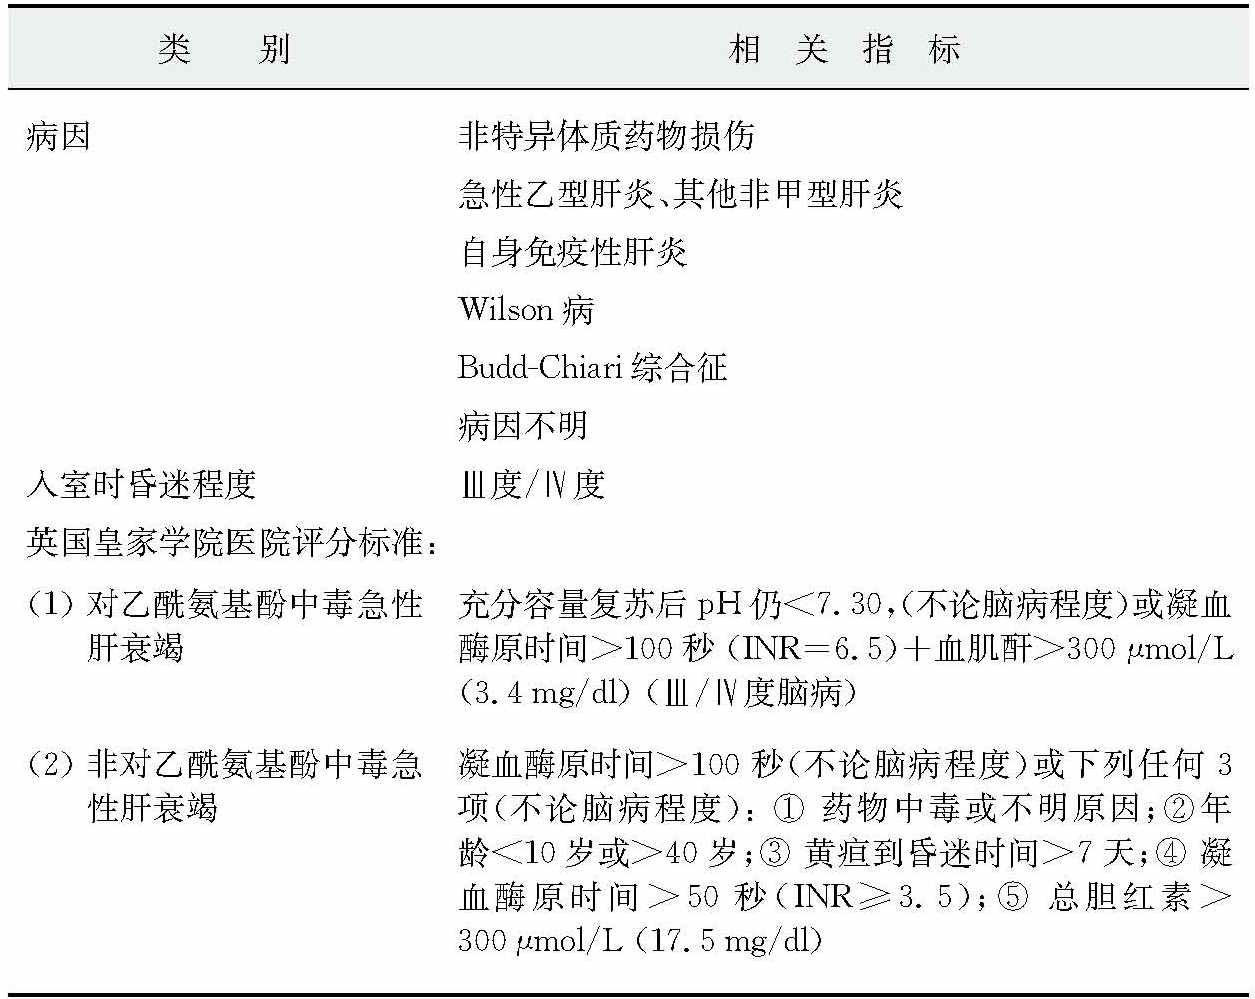
\includegraphics{./images/Image00103.jpg}
\end{table}

\subsubsection{如何理解急性肝衰竭?}

急性肝衰竭一般是指既往无肝病者肝功能受损后短时间内出现严重的凝血障碍和肝性脑病。

1969年Trey等提出爆发性肝衰竭(fulminant hepatic
failure,FHF),是指诊断肝病8周内发生肝性脑病,既往无肝脏病史。1986年Bernuan提议把黄疸出现2周内发生肝性脑病的急性肝衰竭称为爆发性肝衰竭,而把黄疸出现2周至12周内发生的肝衰竭称为亚爆发性肝衰竭(subfulminant
liver failure)。

最近Grady等主张将急性肝衰竭分为3类------

(1)超急性肝衰竭型:黄疸出现1周内发生肝性脑病。该型脑水肿发生率高,存活率也高。多见年轻人。

(2)急性肝衰竭型:黄疸出现1~4周发生肝性脑病。脑水肿发生率较高,但存活率低。

(3)亚急性肝衰竭型:黄疸持续4周后发生肝性脑病,多见老年人。脑水肿发生率低,以腹水多见,病死率高。

该分类对原位肝移植适应证的确定是有意义的。后两类是肝移植的适应证。

然而这些曾经用于描述急性肝衰竭的名词均不够全面,用于区分病程长短的名词并不比病因有更好的预后判断价值。例如,超急性的病例预后可能更好,但这只是因为大多数超急性的病例是由于对乙酰氨基酚中毒造成的。近年来急性肝衰竭最被广泛认可的定义为:预先不存在肝硬化的患者出现凝血异常(通常INR≥1.5)、不同程度的意识改变(肝性脑病),并且疾病持续时间少于26周。Wilson病患者、垂直获得性HBV感染者或自身免疫性肝炎的患者尽管存在肝硬化的可能,但如果被诊断的时间少于26周,也可包括在急性肝衰竭之内。该定义系由美国肝脏病学会(The
American Association for the Study of Liver Diseases)于2005年提出
\protect\hyperlink{text00019.htmlux5cux23ch26-18}{\textsuperscript{{[}26{]}}}
。美国肝脏病学会还规定,如为母婴传播乙型肝炎或自身免疫性肝炎,尽管有肝硬化可能,只要本次起病<26周,仍可诊断急性肝衰竭。此外,慢性乙型肝炎的再活化所致急性肝衰竭亦可纳入,这是因为此时导致肝衰竭的原因是急性发病和肝坏死为主,因此认为,急性肝衰竭应发生于“正常个体”,应理解为原有肝病处于相对静止阶段。据此,HBV无症状携带者和慢性乙型肝炎发生肝炎突发或再活化、慢性乙型肝炎基础上发生HDV重叠感染所致肝衰竭均可列入急性肝衰竭。

\subsubsection{急性肝衰竭及肝性脑病的主要临床表现有哪些?}

急性肝衰竭起病急,进展快,早期症状缺乏特异性,可能仅有恶心、呕吐、腹痛、脱水等表现。随后可出现黄疸、凝血功能障碍、酸中毒或碱中毒、低血糖和昏迷等。精神活动障碍与凝血酶原时间延长是急性肝衰竭的特征。根据意识改变的程度可将肝性脑病分为四级(表\ref{tab13-2})。

\begin{table}[htbp]
\centering
\caption{肝性脑病分级}
\label{tab13-2}
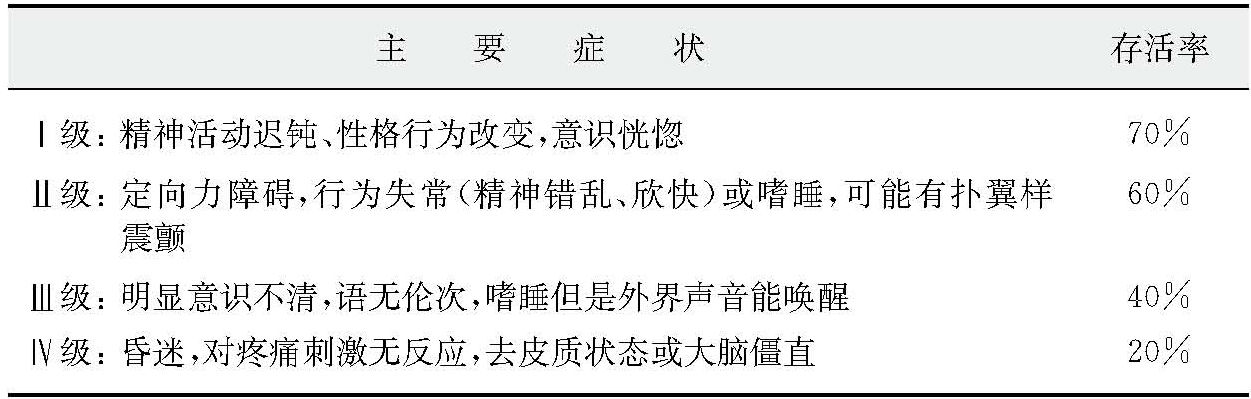
\includegraphics{./images/Image00104.jpg}
\end{table}

\subsection{急性肝衰竭的防治}

\subsubsection{如何防治肝性脑病引起的颅内压增高?}

脑水肿和颅内压增高一直被认为是急性肝衰竭最危险的并发症,发展至颞叶沟回疝则很快危及患者生命,其病理机制尚未完全明了,可能与脑血管自动调节机制紊乱导致脑灌注增加、脑内渗透压改变、炎症反应等多种因素相关。

颅内压增高的临床征兆有:①收缩期高血压(持续性或阵发性);②心动过缓;③肌张力增高,角弓反张,去脑样姿势;④瞳孔异常(对光反射迟钝或消失);⑤脑干型呼吸,呼吸暂停。脑水肿与颅压升高的发生和肝性脑病严重程度相关,Ⅰ~Ⅱ度肝性脑病很少有脑水肿,发展至Ⅲ度和Ⅳ度则脑水肿危险性分别增加到25%~35%和65%~75%
\protect\hyperlink{text00019.htmlux5cux23ch27-18}{\textsuperscript{{[}27{]}}}
,不同程度脑病可采取不同防治方法。

(1)Ⅰ~Ⅱ度肝性脑病 Ⅰ度肝性脑病患者可在内科病房安静环境下接受有经验的护理,尽量减少激惹和刺激,仔细观察患者意识状态,如进展为Ⅱ度脑病则应立即转入重症医学科,同时行头颅CT检查除外颅内出血引起的意识改变,此时应尽量避免使用镇静剂,如患者过度躁动可给予小剂量短效安定类药物。

(2)Ⅲ~Ⅳ度肝性脑病 如肝性脑病进展至Ⅲ或Ⅳ度,应抬高患者头部30°,并进行气管内插管以维持气道通畅,若需要应用镇静剂,可考虑给予小剂量异丙酚,此药可能减低脑血流量,应密切监测患者血液动力学参数、肾功能、血糖、电解质和酸碱平衡及颅内压水平,患者床头抬高30°是为了尽量减少刺激、用力或类似Valsalva样动作而增加颅内压,在给予气管吸痰时建议气道滴入利多卡因。

(3)乳果糖 近来认为血氨增高与脑水肿有关,给动物输入氨可造成脑水肿,人体内动脉血氨超过200μg/dl与脑疝形成有很强的相关性,以及之前治疗肝硬化患者肝性脑病的经验,推荐急性肝衰竭患者给予肠内使用乳果糖降低血氨水平治疗和预防脑水肿进一步加重。美国急性肝衰竭研究学组(USALFSG)临床回顾比较了两组急性肝衰竭患者,发现乳果糖治疗组生存时间稍长,但脑病严重程度和疾病最终结局无显著差异
\protect\hyperlink{text00019.htmlux5cux23ch28-18}{\textsuperscript{{[}28{]}}}
。急性肝衰竭患者使用乳果糖唯一不利方面在于有些患者会加重腹部胀气,为以后肝移植手术增加难度。

(4)控制癫痫发作 癫痫发作是颅压增高及可能发展为肝性脑病的征象,应该使用苯妥英钠和低剂量的苯二氮䓬
类药物处理,其他任何镇静剂均不推荐使用。癫痫发作可急剧增高颅内压并引起大脑缺氧进一步加重脑水肿。一些专家提倡在有不明显癫痫时预防使用苯妥英钠,一个小样本随机对照试验显示急性肝衰竭患者预防应用苯妥英钠对整体存活率无影响,但尸检结果脑水肿有显著减轻。最近一项临床试验结果提示预防癫痫对脑水肿和病死率均无影响,对于预防使用苯妥英钠,仍需进一步验证
\protect\hyperlink{text00019.htmlux5cux23ch29-18}{\textsuperscript{{[}29{]}}}
\textsuperscript{~}
\protect\hyperlink{text00019.htmlux5cux23ch32-18}{\textsuperscript{{[}32{]}}}
,因此目前尚不推荐预防使用苯妥英钠。

\subsubsection{急性肝衰竭患者有必要进行颅内压监测吗?}

急性肝衰竭患者是否需颅内压监测一直是一个有争议的问题,调查结果显示美国有半数以上中心使用颅内压监测,否则不能早期发现脑水肿,颅压增高的临床征象有高血压、心动过缓、呼吸不规则三联征,这些表现并不是每个患者都有,并且一些其他神经系统改变如瞳孔扩大、去大脑僵直只有在颅压增高程度很明显时才会出现。CT并不能很好反映脑水肿特别是在早期,其他监测手段(如经颅多普勒、近红外线分光法)尚未证实能有效反映颅内压的临床价值。

监测的目的是早期发现颅内压升高,及时处理,保障脑灌注压,减少脑疝形成可能,维持神经系统功能,争取肝脏功能恢复或肝移植的机会。对于列入等待肝移植的患者应行颅内压监测,因为血液动力学改变可以引起脑压力参数的剧烈波动,许多中心都认为难治性颅压升高和脑灌注压下降都是移植禁忌证。有文献报道颅内压监测可以安全地提供有效的信息,甚至能延长生存时间,但尚无对照试验显示对整体生存率有益。美国一项262名肝移植患者的研究结果显示,使用有创颅压监测的主要并发症是局部感染和出血,3.8%的患者使用硬脑膜外颅压检测后出现并发症(其中1例发生致死性出血),认为使用硬脑膜下或脑实质内感应装置会增加并发症的发生,积极纠正凝血紊乱包括使用重组活性Ⅶ因子可能为使用颅内压监测装置增加机会。

\subsubsection{急性肝衰竭患者颅压升高的治疗措施有哪些?}

颅内压监测中最重要的参数是颅内压和脑灌注压,颅内压应维持在20~25mmHg,脑灌注压维持在50~60mmHg,对神经系统预后有帮助,因此治疗的目的在于降低颅内压,并提高循环血压维持脑灌注压在50~60mmHg水平。

(1)甘露醇 颅内压监测出现神经体征(如去大脑状态、瞳孔异常等症状)提示颅内压升高,应使用渗透性利尿剂,有对照试验结果显示急性肝衰竭患者静脉使用甘露醇对改善脑水肿有短期效果并可以提高生存率,因此推荐急性肝衰竭颅压升高患者使用负荷剂量0.5~1g/kg的甘露醇,如血清渗透压未超过320mosm/L可以重复1~2次,对于有肾功能损害的患者可能会产生容量负荷过重,从而需要增加透析治疗,过多使用甘露醇也会产生高渗透压和高钠血症,所以对于肾功能损害的患者不建议预防使用甘露醇。

(2)过度通气 过度通气降低动脉血二氧化碳分压至25~30mmHg可以通过血管收缩降低脑血流,从而快速降低颅内压,但其作用维持时间很短。一项随机对照试验结果提示,急性肝衰竭患者连续过度通气可以延迟脑疝出现时间,但对脑水肿和患者生存率并无影响。过度通气引起的脑血管收缩也有加重脑缺氧促进脑水肿的可能,因此认为预防性过度通气并无益处。如果输注甘露醇仍不能降低危及生命的颅压升高,可以暂时实施过度通气预防脑疝形成,但是不建议常规使用过度通气。

(3)高张钠 最近一项对伴严重肝性脑病的急性肝衰竭患者的对照试验显示,使用高张盐水使血钠维持在145~155mmol/L,可以降低颅内压,但对生存率无明显影响。预防使用高张钠是否能通过改善颅内压升高而改善预后,仍需大样本试验确证。

(4)巴比妥类药物 当严重颅压升高对其他治疗方法无反应时,使用巴比妥类药物(如硫喷妥钠或戊巴比妥)可以降低颅内压,但需要同时监测并维持足够的平均动脉压。

(5)皮质类固醇 皮质类固醇激素常用于脑肿瘤和中枢神经系统感染引起的颅内压增高,但对于急性肝衰竭引起的颅内压增高,随机对照试验结果显示对改善脑水肿和生存率均无作用。

(6)低温疗法 使体温降低至32~34℃可能会缓解急性肝衰竭患者的颅内压增高。动物实验显示,低温阻止颅压进一步增高的机制可能与减少脑血管充血、影响脑内氨和糖代谢有关,少数临床实验结果显示低温疗法对急性肝衰竭患者有益,但缺乏随机对照设计。体温过低可增加感染率、凝血紊乱、心律失常等危险,应予以重视。

\subsubsection{如何对急性肝衰竭患者进行常规治疗及器官支持?}

急性肝衰竭的临床过程为进行性多器官功能衰竭,除中毒引起者可用解毒药外,其余情况均无特效疗法。治疗目标是生命支持,期望肝功能恢复或有条件时进行肝移植。急性肝衰竭患者需要加强防治的主要并发症及对策见表\ref{tab13-3}。

\begin{table}[htbp]
\centering
\caption{急性肝衰竭患者需要加强防治的主要并发症及对策}
\label{tab13-3}
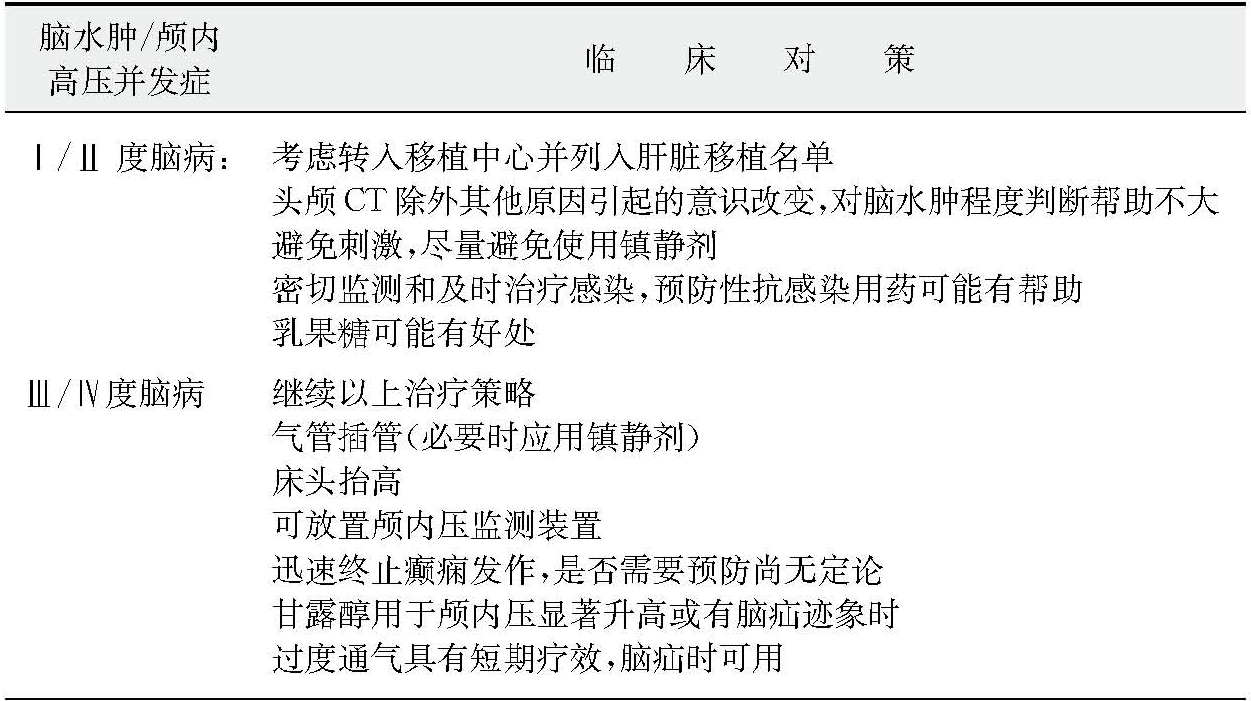
\includegraphics[width=\textwidth,height=\textheight,keepaspectratio]{./images/Image00106.jpg}
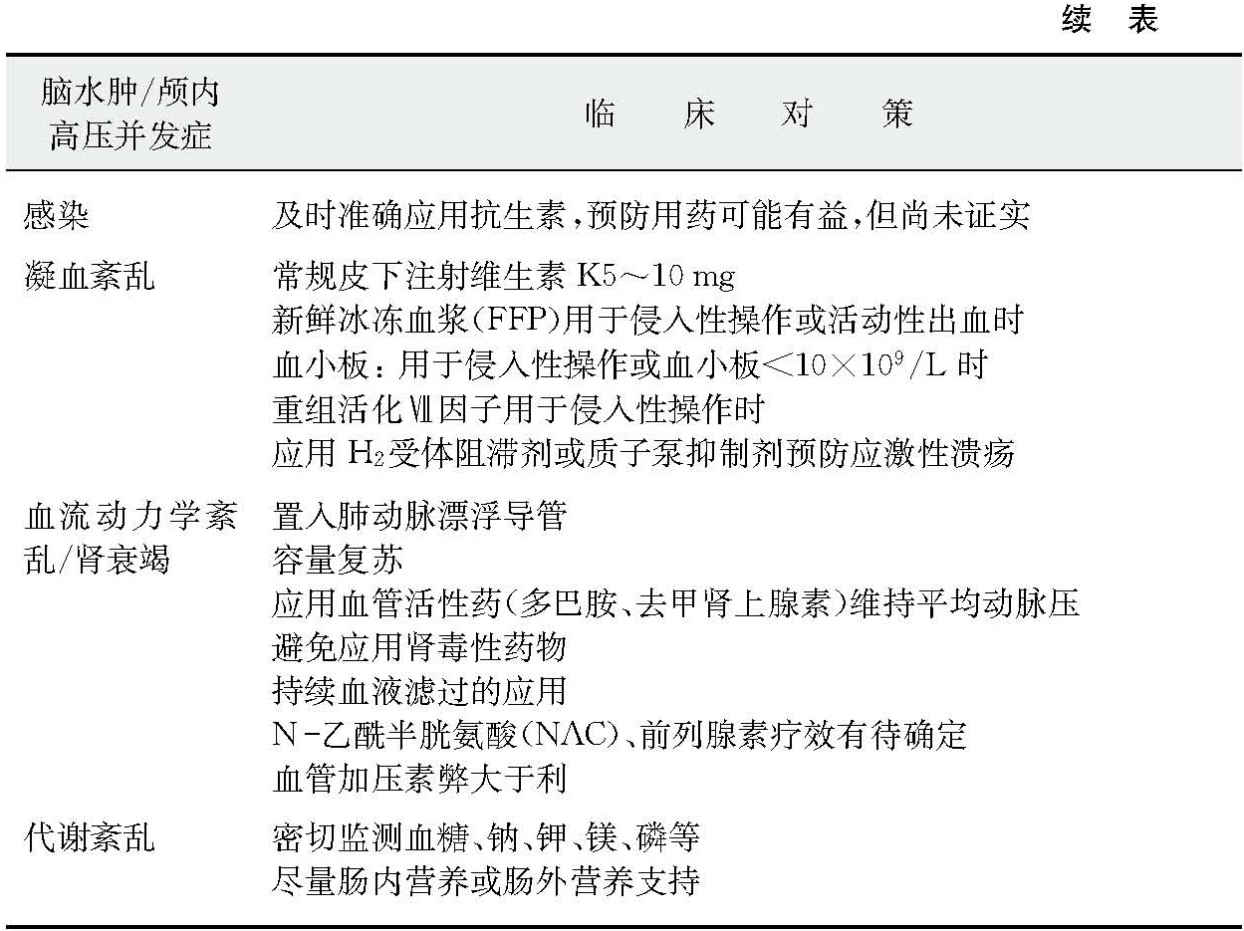
\includegraphics[width=\textwidth,height=\textheight,keepaspectratio]{./images/Image00107.jpg}
\end{table}


(1)一般措施 密切观察患者精神状态、血压、尿量。常规给予H\textsubscript{2}
受体拮抗剂以预防应激性溃疡。皮质类固醇、肝素、胰岛素、胰高血糖素无明显效果。抗病毒药未被用于治疗急性肝衰竭,近期有报告可试用拉米夫定治疗急性肝衰竭者。

(2)肝性脑病和脑水肿 详见上节。

(3)感染问题 所有急性肝衰竭患者均有感染细菌、真菌甚至脓毒症的风险,可能导致肝移植不能进行或术后恢复困难。可考虑预防性使用抗生素和抗真菌药物以降低感染发生率,但是没有证据提示抗菌治疗对疾病的最终结局有改善。部分(30%以上)并发感染者无典型临床征兆(如发热、白细胞增多等),意识状态改变经常预示着感染的发生,所以应提高警觉。应定期拍X线胸片,取痰、血、尿进行细菌和真菌培养以密切监测感染的发生,早期发现感染并给予积极治疗是改善预后的关键。

(4)凝血功能障碍 急性肝衰竭患者几乎都有凝血功能障碍,并发出血的风险很高。由于凝血因子合成能力降低,同时凝血因子和血小板消耗增多,因此血小板常在10×10\textsuperscript{9}
/L以下。预防性应用新鲜冰冻血浆并不能改善预后,只有在明显出血、准备外科手术、侵入性检查或凝血严重紊乱(如INR>7)时才用新鲜冰冻血浆或其他特殊凝血因子浓缩物。血小板少于10×10\textsuperscript{9}
/L者,可能需要输血小板。输血还存在着风险,补充血浆(尤其是库存血浆而非新鲜冰冷血浆)对凝血改善的价值有限,且可使血容量增加而加重颅内高压。

(5)消化道出血 消化道出血是急性肝衰竭常见的并发症,一项多中心调查发现机械通气>48小时、凝血异常是导致重症医学科患者胃肠道出血的独立危险因素,其他危险因素包括肝衰竭、肾衰竭、脓毒血症等,因此,急性肝衰竭是消化道出血的高危情况。

预防性应用H\textsubscript{2}
受体拮抗剂和硫糖铝,可显著降低上消化道出血的发生率。与硫糖铝比较,H\textsubscript{2}
受体阻断剂在防止出血方面可能更加有效,但需经进一步的证明;硫糖铝可作为二线预防性用药。一般推荐急性肝衰竭患者应接受H\textsubscript{2}
受体阻断剂或质子泵抑制剂(或用硫糖铝作为二线用药)治疗,以预防因应激性溃疡导致的酸相关性胃肠道出血。

(6)血液动力学紊乱/肾衰竭 急性肝衰竭患者血液动力学紊乱的机制尚未完全阐明。由于常同时伴有颅内高压和肾脏功能不全,因此及时纠正血液动力学紊乱显得尤为重要,但也具有一定难度,急性肝衰竭患者血液动力学紊乱的病理生理很多方面类似肝硬化肝肾综合征患者,此时对于肾脏的保护十分重要。入院时患者就可能出现血管内容量不足甚至需要液体复苏,其原因包括意识状态障碍导致饮食摄入减少、液体向血管外间隙渗出、消化道出血等。患者通常还会伴有血管阻力下降,液体复苏后血流动力学仍不稳定者应考虑插入肺动脉漂浮导管,加强监测、指导治疗,液体复苏以胶体为主(如白蛋白等),适当补充葡萄糖维持血糖在80~110mg/dl范围内。

充分补液和抗感染治疗后血压仍不能纠正应该使用血管活性药(如肾上腺素或去甲肾上腺素和多巴胺),维持平均动脉压在50~60mmHg以上,以保证肾脏灌注。

急性肝衰竭患者常由于脱水、肝肾综合征、急性肾小管坏死或对乙酰氨基酚及其他药物的直接损害导致急性肾衰竭,增加病死率,因此应尽一切努力保护肾脏,包括维持血液动力学稳定、避免使用诸如氨基糖苷类和非甾体类抗炎药等具有肾损害药物、早期发现并积极控制感染,如需要透析应优先选择持续性肾脏替代治疗,随机对照试验表明持续治疗比间断治疗对心血管系统、脑灌注压稳定更为有益。静脉使用血管造影剂具有诱导肾功能损害的作用,应慎重使用。前列腺素和N-乙酰半胱氨酸(N-acetylcysteine,NAC)对维持血液动力学稳定保护肾脏方面的作用,目前仍有争议。特利加压素和垂体加压素能有效治疗肝硬化肝肾综合征,但最近小样本研究认为即便是很小剂量的特利加压素也可引起脑血流增加,并且可能加重颅内高压,因此,不推荐血管加压素用于急性肝衰竭患者。

(7)代谢紊乱 急性肝衰竭患者常见的代谢紊乱包括低血糖、代谢性酸中毒、代谢性碱中毒及电解质紊乱,治疗基础疾病是纠正代谢紊乱的关键,急性肝衰竭伴肝性脑病的患者出现低血糖时症状隐匿,易漏诊,应加强监测,并适当补充葡萄糖,大量补糖会导致肝脏脂肪化,加重肝脏负担。低磷、低镁、低钾血症也较为常见,应定时监测、及时补充。对乙酰胺基酚中毒时常出现代谢性酸中毒,pH<7.3时,死亡高达90%,非扑热息痛引起的急性肝衰竭多为碱中毒,可能与肝脏合成尿素障碍有关。

(8)营养支持 营养支持十分重要,应早期给予患者肠内营养,不应该严格限制蛋白摄入,大多数患者60g蛋白/天比较合理,支链氨基酸并不优于其他肠内制剂,无法实施肠内营养时可采取静脉营养,但后者可增加感染发生几率(特别是真菌感染),肠内外营养还可以减少危重症患者应激性溃疡引起的消化道出血。

\subsubsection{肝脏移植有什么适应证及禁忌证?}

肝移植(orthotopic liver
transplantation,OLT)是目前治疗急性肝衰竭最有效的方法,其1年生存率可达80%。但掌握肝移植的时机是困难的。移植前肝病越重,手术病死率越高。因此,肝移植患者选择非常重要,目前通常采用英国O'Grady(1989年)的伦敦标准
\protect\hyperlink{text00019.htmlux5cux23ch33-18}{\textsuperscript{{[}33{]}}}
(表\ref{tab13-4})。

\begin{table}[htbp]
\centering
\caption{爆发性肝衰竭肝移植指征}
\label{tab13-4}
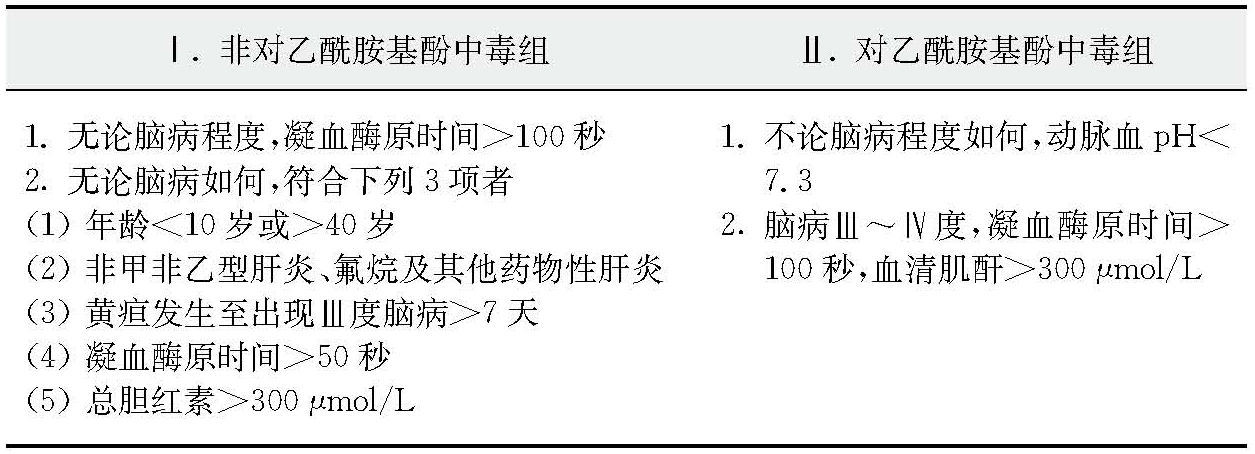
\includegraphics{./images/Image00108.jpg}
\end{table}

出血、肾衰竭、高胆红素血症和脑水肿是影响移植预后的重要因素。败血症是移植术后主要死亡原因。顽固性颅内高压、脓毒血症、永久性脑损害、低血压、ARDS应作为肝移植绝对禁忌证。

\subsubsection{什么是人工肝支持系统?}

人工肝支持系统(artifical liver surpport
system,ALSS)是指通过体外机械、理化或生物性装置暂时辅助或替代衰竭肝脏功能的治疗方式,及时有效的功能支持将为肝细胞恢复或肝脏移植争取时机。

1950年,Merrill首先将血液透析应用于肝衰竭的治疗。1956年,Sorrention证明新鲜肝组织匀浆能代谢酮体、巴比妥和氨,首次提出“人工肝”的概念,同年日本杉浦光雄等人研制出了简单的人工肝脏。1958年,Kimoto首次应用人工肝救治了1例肝硬化肝性脑病患者。他将4条狗的肝与交叉血透器并联,与离子交换树脂串联,方法繁琐。上世纪70年代,血液净化技术推动了非生物人工肝的发展。80年代开始,随着肝细胞分离、培养技术的日趋成熟,掀起了生物人工肝的研究高潮,对肝细胞培养、功能维持、生物反应器的设计等进行了广泛深入的研究。

理想的替代装置应包括解毒、代谢和合成等肝脏所有主要功能。迄今,世界各地已经研制出各种不同的肝支持系统,但均未得到肯定有效的证据。按照人工肝组成及性质一般可分为两大类:

(1)非生物人工肝支持系统 该系统大多以解毒为主,部分兼有补充生物活性物质作用,主要包括血液透析(hemodialysis)、血液滤过(hemofiltration)、血液灌流(hemoperfusion)、血浆置换(plasmaexchange)、分子吸附再循环系统(molecular
adsorbents recycling
system,MARS)等。能通过透析、过滤及吸附等方法净化血液,排除肝衰竭患者血液中过多的毒性产物,包括氨、细胞因子(如TNFα、IL-6)、酚、脂肪酸及内毒素等,有效地改善患者术前的内环境紊乱,降低胆红素,纠正水、电解质紊乱。合理的人工肝支持治疗可明显改善患者的意识状态,有效地减低血氨水平。

(2)生物人工肝支持系统 该系统利用外源性的具有部分或全部肝细胞生物活性的细胞作为生物反应细胞,在体外或体内替代部分或全部肝脏功能。与非生物人工肝单纯清除体内毒素不同,生物人工肝不仅能通过对毒素的代谢转化清除毒素,而且能合成生物活性物质如葡萄糖、凝血因子、白蛋白等血浆蛋白参与机体功能活动,并调节体内血糖等代谢活动。由于目前生物人工肝技术尚不成熟,故一般与非生物人工肝联合使用,以达到更全面的肝脏支持作用。初期临床对照试验报告显示这种人工肝支持系统对临床结局无改善作用。最近的一个多中心临床试验发现采用猪肝细胞为基础的生物型人工肝治疗的急性肝衰竭患者组短期存活率有提高,但是还需要进一步的研究来证实这一结果
\protect\hyperlink{text00019.htmlux5cux23ch34-18}{\textsuperscript{{[}34{]}}}
\textsuperscript{,}
\protect\hyperlink{text00019.htmlux5cux23ch35-18}{\textsuperscript{{[}35{]}}}
。

\subsubsection{如何评价血液滤过在急性肝衰竭中的治疗作用?}

血液滤过是模拟正常肾小球的滤过作用,将血液通过高通透性膜制成的滤器,通过跨膜压使水分经滤过膜进入滤液,然后补充与细胞外液相似的电解质溶液,达到排除体内废物和过多水分的目的。1907年,Bechhold就提出模仿肾脏滤过功能清除人体过量的水分和溶质。1928年Brull设计了简易超滤器并用狗进行了初步实验。1947年,Malinow等首次用人工肾进行超滤实验。1955年Alwall应用单纯超滤治疗水肿。1967年Henderson等报道用多种渗透膜清除过多液体并补充置换液。1973年血液滤过技术正式用于临床。1977年在赫尔辛基召开的第14届欧洲透析移植协会大会上报道了该技术在肝病方面的应用。1979年Denis等治疗10例急性肝衰竭伴Ⅳ度肝性脑病,平均治疗92小时,50%存活。

由于急性肝衰竭时患者迅速出现肝性脑病、黄疸、凝血障碍、内环境紊乱、循环、呼吸衰竭,肾衰竭等并发症,可以直接导致患者死亡,有效及时的血液滤过有利于清除体内毒素、改善意识、清除体内多余水分,改善组织水肿、缓慢纠正低钠血症,以免引起渗透性脱髓鞘综合征,维持电解质及酸碱平衡、营养支持,提供代谢底物、循环支持,保证组织灌注,赢得时机,等待肝脏恢复或进行肝移植手术。

肝移植由于手术时间较长、术中的无肝期、排斥反应、感染等原因,术后的并发症种类很多,包括原发性移植肝功能障碍、术后出血、凝血功能障碍、门静脉栓塞、下腔静脉梗阻、胆漏、胆道梗阻、高胆红素血症以及各种类型的内科并发症如心肺功能不全、水电解质平衡紊乱及肾衰竭等。此时可以通过血液滤过有效地改善肝移植术后早期患者的生理紊乱状况。移植术后出现急性排斥反应时,移植肝受到破坏,功能低下,在使用免疫抑制疗法的同时行血液滤过联合其他人工肝支持系统治疗,去除抗原及免疫复合物,帮助渡过排斥反应期,有利于移植肝功能的恢复。

\subsubsection{如何评价血浆置换在急性肝衰竭治疗中的作用?}

1914年Abel首次提出,将患者血液抽出,沉淀后去除血浆,剩余成分回输患者。由于技术和安全性的限制,未受到重视。1959年,Waldenstrom将血浆置换应用于临床。20世纪60年代出现间断性血浆分离机。早期常用的血浆分离方法是封闭的离心式血浆分离器,1978年出现了膜式血浆分离装置,用高分子聚合物制成的空心纤维型或平板型滤器,膜孔可准许血浆滤过,但能阻挡所有的细胞成分,使血浆置换在技术上更加简化和实用。

常用的方法是将患者的血液抽出来,分离血浆和细胞成分,弃去血浆,而把细胞成分以及所补充白蛋白、血浆及平衡液等回输体内,以达到清除致病介质的治疗目的。目前,随着技术的不断进步,可选择性分离出某一类或某一种血浆成分从而能够选择性或特异性地清除致病介质,进一步提高了疗效,节省新鲜血浆和白蛋白,减少并发症的发生。

血浆置换的缺点是潜在的感染(目前检测手段未能发现的致病原、HIV等)、过敏、枸橼酸盐中毒等。由于需要反复实施血浆置换以清除有害物质,所需血浆量较大、成本高、血制品使用风险增加。

血浆置换是目前较为成熟的肝脏替代疗法,尽管各种生物型和非生物型人工肝技术快速发展,但血浆置换仍是目前肝衰竭患者的主要和基本人工肝治疗方法。

\subsubsection{如何评价分子吸附再循环系统在急性肝衰竭治疗中的作用?}

分子吸附循环系统(MARS)基本构想最先由Stange等于1993年设计,它由一种可以结合白蛋白的高通量聚砜膜滤器及其他循环系统组成。现在使用的分子吸附循环系统主要由血液循环系统、白蛋白循环再生系统和透析循环系统三部分组成。使用时,血液循环系统是将血液从患者体内引出,经过特制的透析器,透析器内中空纤维管一侧为含有毒素的血液,另外一侧为白蛋白透析液,它们通过特制的中空纤维膜结构交换物质,从而达到解毒作用。分子吸附循环系统透析膜只有普通膜厚度的1/100至1/500,膜的总面积超过2m\textsuperscript{2}
,该膜的特殊性在于可以有效清除血液里一些与白蛋白结合的大分子毒素物质。白蛋白循环再生系统主要是通过对透析液一侧的白蛋白溶液进行透析、吸附,从而恢复白蛋白的功能。透析循环系统是常规的透析装置,可以由常规的透析机完成,主要作用是透析掉白蛋白溶液中的小分子量的毒性物质。

在行分子吸附循环过程中,小分子量的毒素也可以被透析清除。Stange等采用分子吸附循环系统进行了清除地西泮类物质的实验研究,他们将200μg地西泮物质加入1L人体血浆中,以常规的碳酸氢盐血液透析作为对照组,血浆流量150ml/分,透析液流量1000ml/小时。结果分子吸附循环系统的地西泮物质清除率为50%,而对照组仅为7%。一项应用分子吸附循环系统的临床试验中,13例患者经分子吸附循环系统治疗,9例存活,患者的肝功能有所改善,肝性脑病的严重程度亦下降。针对酒精性肝硬化所致的肝衰竭的临床研究中,分子吸附循环系统可使患者的病情得以稳定。该组26例患者,治疗前的血清胆红素≥256.5μmol/L,肝性脑病Ⅱ度以上,其中10例患者存在肝肾综合征,19例伴有系统性炎性综合征、脓毒症和继发并发症。经分子吸附循环系统治疗后,患者的血清胆红素、胆酸和肝性脑病的等级均显著下降,肝脏合成作用(胆碱酯酶、凝血酶原时间)、肾功能异常和血压异常也有所改善,有13例患者未行肝移植而病愈出院。

大量的研究表明,分子吸附循环系统不仅可以有效清除体内小分子量的毒性物质,而且也可以清除机体内与白蛋白结合的大分子毒素,大大改善了肝功能状态。实验证明这一方法能有效去除非结合胆红素、游离脂肪酸、芳香族氨基酸及具高蛋白结合率的药物等。而一些具有生理活性的大分子蛋白质如白蛋白、α\textsubscript{1}
糖蛋白、α\textsubscript{1}
抗胰蛋白酶、α巨球蛋白、转铁蛋白等则不受影响。Novelliet等用分子吸附循环系统治疗了39例急性肝衰竭的患者,结果显示血胆红素由24.4mg/dl降至15.7mg/dl,血氨由263.8μmol/L降至175.5μmol/L。大多数患者经分子吸附循环系统治疗后,血液动力学和神经症状改善,尤其是中毒性肝衰竭的治疗结果令人鼓舞。另外,还发现肝性脑病及脑水肿改善,但平均动脉压和肌酸没有明显变化。有个别报道运用分子吸附循环系统治疗肝窦状核变性所致的急性肝衰竭,血铜明显下降。分子吸附循环系统治疗的唯一并发症是血小板减少。

\begin{center}\rule{0.5\linewidth}{\linethickness}\end{center}

参考文献

\protect\hyperlink{text00019.htmlux5cux23ch1-18-back}{{[}1{]}}
.Hoofnagle JH,Carithers RL,Sapiro C,Ascher N.Fulminant hepatic
failure:summary of a workshop.HEPATOLOGY 1995;21:240-252.

\protect\hyperlink{text00019.htmlux5cux23ch2-18-back}{{[}2{]}}
.Ostapowicz GA,Fontana RJ,Schiodt FV,Larson A,Davern TJ,Han SH,et
al.Results of a prospective study of acute liver failure at 17 tertiary
care centers in the United States.Ann Intern Med 2002;137:947-954.

\protect\hyperlink{text00019.htmlux5cux23ch3-18-back}{{[}3{]}} .Sato
RL,Wong JJ,Sumida SM,Marn RY,Enoki NR,Yamamoto LG.Efficacy of
superactivated charcoal administration late(3 hours)after
acetaminophen overdose.Am J Emerg Med 2003;21:189-191.

{[}4{]}.Sterling RK,Luketic VA,Sanyal AJ,Shiffman ML.Treatment of
fulminant hepatic failure with intravenous prostaglandin E1.Liver
Transpl Surg 1998;4:424-431.

\protect\hyperlink{text00019.htmlux5cux23ch5-18-back}{{[}5{]}} .Walsh
TS,Hopton P,Philips BJ,Mackenzie SJ,Lee A.The effect of
N-acetylcysteine on oxygen transport and uptake in patients with
fulminant hepatic failure.HEPATOLOGY 1998;27:1332-1340.

\protect\hyperlink{text00019.htmlux5cux23ch6-18-back}{{[}6{]}}
.Kjaergard LL,Liu J,Als-Nielsen B,et al.Artificial and
bioartificial support systems for acute and acute-on-chronic liver
failure:a systematic review.JAMA,2003,289:217-222.

\protect\hyperlink{text00019.htmlux5cux23ch7-18-back}{{[}7{]}} .Stevens
C,Busuttil RW,Han S,et al.An interim analysis of a phase Ⅱ/Ⅲ
prospective randomized multicenter controlled trial of the Hepat Assist
Bioartificial Liver Support System for the treatment of fulminant
hepatic failure {[}abstract{]}.Hepatology.2001;34:299A.

\protect\hyperlink{text00019.htmlux5cux23ch8-18-back}{{[}8{]}} .Benson
K,Hartz AJ.A comparison of observational studies and
randomized,controlled trials.N Engl J Med.2000;342:1878-1886.

\protect\hyperlink{text00019.htmlux5cux23ch9-18-back}{{[}9{]}} .Concato
J,Shah N,Horwitz RI.Randomized,controlled trials,observational
studies,and the hierarchy of research designs.N Engl J
Med.2000;342:1887-1892.

\protect\hyperlink{text00019.htmlux5cux23ch10-18-back}{{[}10{]}} .Jiang
YS,Chen YM,Yao JL,et al.Evaluation of the therapeutic effect of
artificial liver support system on severe viral hepatitis.Chin J Intern
Med.2000;39:115-117.

\protect\hyperlink{text00019.htmlux5cux23ch11-18-back}{{[}11{]}}
.Mitzner SR,Stange J,Klammt S,et al.Extracorporeal detoxification
using the molecular adsorbent recirculating system for critically ill
patients with liver failure.J Am Soc Nephrol.2001;12(suppl
17):S75-S82.

{[}12{]}.He JQ,Chen CY,Deng JT,et al.Clinical study on the
treatment of fatal hepatitis with artificial liver support system.Chin
Crit Care Med.2000;12:105-108.

\protect\hyperlink{text00019.htmlux5cux23ch13-18-back}{{[}13{]}}
.Heemann U,Treichel U,Loock J,et al.Albumin dialysis in cirrhosis
with superimposed acute liver injury:a prospective,controlled
study.Hepatology.2002;36:949-958.

\protect\hyperlink{text00019.htmlux5cux23ch14-18-back}{{[}14{]}}
.Schiodt FV,Davern TA,Shakil O,McGuire B,Samuel G,Lee WM.Viral
hepatitis-related acute liver failure.Am J Gastroenterol
2003;98:448-453.

\protect\hyperlink{text00019.htmlux5cux23ch15-18-back}{{[}15{]}}
.Khuroo MS,Kamili S.Aetiology and prognostic factors in acute liver
failure in India.J Viral Hepatol 2003;10:224-231.

\protect\hyperlink{text00019.htmlux5cux23ch16-18-back}{{[}16{]}} .Lee
WM.Drug-Induced Hepatotoxicity.N Engl J Med 2003;349:474-485.

\protect\hyperlink{text00019.htmlux5cux23ch17-18-back}{{[}17{]}} .Vale
JA,Proudfoot AT.Paracetamol(acetaminophen)poisoning.Lancet
1995;346:547-552.

\protect\hyperlink{text00019.htmlux5cux23ch18-18-back}{{[}18{]}}
.Rengstorff DS,Osorio RW,Bonacini M.Recovery from severe hepatitis
caused by mushroom poisoning without liver transplantation.Clinical
Gastroenterology and HEPATOLOGY 2003;1:392-396.

{[}19{]}.Enjalbert F,Rapior S,Nouguier-Soule J,Guillon S,Amouroux
N,Cabot C.Treatment of amatoxin poisoning:20-year retrospective
analysis.J Toxicol Clin Toxicol 2002:40:715-757.

\protect\hyperlink{text00019.htmlux5cux23ch20-18-back}{{[}20{]}}
.Broussard CN,Aggarwal A,Lacey SR,Post AB,Gramlich T,Henderson
M,et al.Mushroom poisoning---from diarrhea to liver
transplantation.Am J Gastroenterol 2001;96:3195-3198.

\protect\hyperlink{text00019.htmlux5cux23ch21-18-back}{{[}21{]}}
.O'Grady JG,Alexander GJM,Hayllar KM,Williams R.Early indicators of
prognosis in fulminant hepatic failure.Gastroenterology
1989;97:439-455.

\protect\hyperlink{text00019.htmlux5cux23ch22-18-back}{{[}22{]}}
.Bailey B,Amre DK,Gaudreault P.Fulminant hepatic failure secondary
to acetaminophen poisoning:A systematic review and meta-analysis of
prognostic criteria determining the need for liver transplantation.Crit
Care Med 2003;31:299-305.

{[}23{]}.Nagaki M,Iwai H,Naiki T,Ohnishi H,Muto Y,Moriwaki H.High
levels of serum interleukin-10 and tumor necrosis factor-a are
associated with fatality in fulminant hepatitis.J Infect Dis
2000;182:1103-1108.

{[}24{]}.Davern TJ,Polson J,Lalani E,Lee WM and the US ALF Study
Group.Serum phosphate levels as a predictor of clinical outcome in
acetaminopheninduced acute liver failure.HEPATOLOGY 2003,AASLD meeting
abstract.

\protect\hyperlink{text00019.htmlux5cux23ch25-18-back}{{[}25{]}} .Harry
R,Auzinger G,Wendon J.The clinical importance of adrenal
insufficiency in acute hepatic dysfunction.HEPATOLOGY
2002;36:395-402.

\protect\hyperlink{text00019.htmlux5cux23ch26-18-back}{{[}26{]}}
.Polson J,Lee WM.American Association for the Study of Liver
Disease.(AASLD)Position Paper:The Management of Acute Liver
Failure.Hepatology.2005,41:1179-1197.

\protect\hyperlink{text00019.htmlux5cux23ch27-18-back}{{[}27{]}}
.Vaquero J,Chung C,Cahill ME,Blei AT.Pathogenesis of hepatic
encephalopathy in acute liver failure.Semin Liver Disease
2003;23:259-269.

\protect\hyperlink{text00019.htmlux5cux23ch28-18-back}{{[}28{]}} .Alba
L,Hay JE,Angulo P,Lee WM.Lactulose therapy in acute liver failure.J
Hepatol 2002;36:33A.

\protect\hyperlink{text00019.htmlux5cux23ch29-18-back}{{[}29{]}}
.Wijkicks EFM,Nyberg SL.Propofol to control intracranial pressure in
fulminant hepatic failure.Transplant Proc 2002;34:1220-1222.

{[}30{]}.Ellis AJ,Wendon JA,Williams R.Subclinical seizure activity
and prophylactic phenytoin infusion in acute liver failure:a controlled
clinical trial.HEPATOLOGY 2000;32:536-541.

{[}31{]}.Bhatia V,Batra Y,Acharya SK.Prophylactic phenytoin does not
improve cerebral edema or survival in acute liver failure---a controlled
clinical trial.J Hepatol 2004;41:89-96.

\protect\hyperlink{text00019.htmlux5cux23ch32-18-back}{{[}32{]}}
.Vaquero J,Fontana R,Lee W,Blei AT.Outcome of intracranial pressure
monitoring in acute liver failure(ALF)[Abstract].HEPATOLOGY
2004;40(Suppl 1):212A.

\protect\hyperlink{text00019.htmlux5cux23ch33-18-back}{{[}33{]}}
.O'Grady JG,Schalm SW,Williams R:Acute liver failure:Redefining the
syndromes.Lancet 1993;342:273-275.

\protect\hyperlink{text00019.htmlux5cux23ch34-18-back}{{[}34{]}}
.Demetriou AA,Brown RS Jr,Busuttil RW,Fair J,McGuire BM,Rosenthal
P,et al.Prospective,randomized,multicenter,controlled trial of a
bioartificial liver in treating acute liver failure.Ann Surg
2004;239:660-667.

\protect\hyperlink{text00019.htmlux5cux23ch35-18-back}{{[}35{]}}
.Kjaergard LL,Liu J,Adils-Neilsen B,Gluud C.Artificial and
bioartificial liver support systems for acute and acute-on-chronic liver
failure.JAMA 2003;289:217-222.

\protect\hypertarget{text00020.html}{}{}

